\documentclass[]{tufte-handout}

% ams
\usepackage{amssymb,amsmath}

\usepackage{ifxetex,ifluatex}
\usepackage{fixltx2e} % provides \textsubscript
\ifnum 0\ifxetex 1\fi\ifluatex 1\fi=0 % if pdftex
  \usepackage[T1]{fontenc}
  \usepackage[utf8]{inputenc}
\else % if luatex or xelatex
  \makeatletter
  \@ifpackageloaded{fontspec}{}{\usepackage{fontspec}}
  \makeatother
  \defaultfontfeatures{Ligatures=TeX,Scale=MatchLowercase}
  \makeatletter
  \@ifpackageloaded{soul}{
     \renewcommand\allcapsspacing[1]{{\addfontfeature{LetterSpace=15}#1}}
     \renewcommand\smallcapsspacing[1]{{\addfontfeature{LetterSpace=10}#1}}
   }{}
  \makeatother

\fi

% graphix
\usepackage{graphicx}
\setkeys{Gin}{width=\linewidth,totalheight=\textheight,keepaspectratio}

% booktabs
\usepackage{booktabs}

% url
\usepackage{url}

% hyperref
\usepackage{hyperref}

% units.
\usepackage{units}


\setcounter{secnumdepth}{-1}

% citations
\usepackage{natbib}
\bibliographystyle{plainnat}


% pandoc syntax highlighting
\usepackage{color}
\usepackage{fancyvrb}
\newcommand{\VerbBar}{|}
\newcommand{\VERB}{\Verb[commandchars=\\\{\}]}
\DefineVerbatimEnvironment{Highlighting}{Verbatim}{commandchars=\\\{\}}
% Add ',fontsize=\small' for more characters per line
\newenvironment{Shaded}{}{}
\newcommand{\AlertTok}[1]{\textcolor[rgb]{1.00,0.00,0.00}{\textbf{#1}}}
\newcommand{\AnnotationTok}[1]{\textcolor[rgb]{0.38,0.63,0.69}{\textbf{\textit{#1}}}}
\newcommand{\AttributeTok}[1]{\textcolor[rgb]{0.49,0.56,0.16}{#1}}
\newcommand{\BaseNTok}[1]{\textcolor[rgb]{0.25,0.63,0.44}{#1}}
\newcommand{\BuiltInTok}[1]{#1}
\newcommand{\CharTok}[1]{\textcolor[rgb]{0.25,0.44,0.63}{#1}}
\newcommand{\CommentTok}[1]{\textcolor[rgb]{0.38,0.63,0.69}{\textit{#1}}}
\newcommand{\CommentVarTok}[1]{\textcolor[rgb]{0.38,0.63,0.69}{\textbf{\textit{#1}}}}
\newcommand{\ConstantTok}[1]{\textcolor[rgb]{0.53,0.00,0.00}{#1}}
\newcommand{\ControlFlowTok}[1]{\textcolor[rgb]{0.00,0.44,0.13}{\textbf{#1}}}
\newcommand{\DataTypeTok}[1]{\textcolor[rgb]{0.56,0.13,0.00}{#1}}
\newcommand{\DecValTok}[1]{\textcolor[rgb]{0.25,0.63,0.44}{#1}}
\newcommand{\DocumentationTok}[1]{\textcolor[rgb]{0.73,0.13,0.13}{\textit{#1}}}
\newcommand{\ErrorTok}[1]{\textcolor[rgb]{1.00,0.00,0.00}{\textbf{#1}}}
\newcommand{\ExtensionTok}[1]{#1}
\newcommand{\FloatTok}[1]{\textcolor[rgb]{0.25,0.63,0.44}{#1}}
\newcommand{\FunctionTok}[1]{\textcolor[rgb]{0.02,0.16,0.49}{#1}}
\newcommand{\ImportTok}[1]{#1}
\newcommand{\InformationTok}[1]{\textcolor[rgb]{0.38,0.63,0.69}{\textbf{\textit{#1}}}}
\newcommand{\KeywordTok}[1]{\textcolor[rgb]{0.00,0.44,0.13}{\textbf{#1}}}
\newcommand{\NormalTok}[1]{#1}
\newcommand{\OperatorTok}[1]{\textcolor[rgb]{0.40,0.40,0.40}{#1}}
\newcommand{\OtherTok}[1]{\textcolor[rgb]{0.00,0.44,0.13}{#1}}
\newcommand{\PreprocessorTok}[1]{\textcolor[rgb]{0.74,0.48,0.00}{#1}}
\newcommand{\RegionMarkerTok}[1]{#1}
\newcommand{\SpecialCharTok}[1]{\textcolor[rgb]{0.25,0.44,0.63}{#1}}
\newcommand{\SpecialStringTok}[1]{\textcolor[rgb]{0.73,0.40,0.53}{#1}}
\newcommand{\StringTok}[1]{\textcolor[rgb]{0.25,0.44,0.63}{#1}}
\newcommand{\VariableTok}[1]{\textcolor[rgb]{0.10,0.09,0.49}{#1}}
\newcommand{\VerbatimStringTok}[1]{\textcolor[rgb]{0.25,0.44,0.63}{#1}}
\newcommand{\WarningTok}[1]{\textcolor[rgb]{0.38,0.63,0.69}{\textbf{\textit{#1}}}}

% longtable
\usepackage{longtable,booktabs}

% multiplecol
\usepackage{multicol}

% strikeout
\usepackage[normalem]{ulem}

% morefloats
\usepackage{morefloats}


% tightlist macro required by pandoc >= 1.14
\providecommand{\tightlist}{%
  \setlength{\itemsep}{0pt}\setlength{\parskip}{0pt}}

% title / author / date
\title[Web Scrapping in R]{Gathering Data from Websites Using \texttt{R}
Programming language}
\author{John Karuitha}
\date{Monday, July 12, 2021}

\usepackage{booktabs}
\usepackage{longtable}
\usepackage{array}
\usepackage{multirow}
\usepackage{wrapfig}
\usepackage{float}
\usepackage{colortbl}
\usepackage{pdflscape}
\usepackage{tabu}
\usepackage{threeparttable}
\usepackage{threeparttablex}
\usepackage[normalem]{ulem}
\usepackage{makecell}
\usepackage{xcolor}

\begin{document}

\maketitle




\hypertarget{background}{%
\subsection{\texorpdfstring{\textbf{Background}}{Background}}\label{background}}

Have you ever come across some valuable data on a website and wished to
access and use it in your research? \footnote{The author is at Karatina
  University, School of Business, P.O. Box 1957-10101, Karatina, Kenya.}
Did you get discouraged from using data from the internet because
writing down the data by hand and transferring it to a spreadsheet
seemed daunting? \footnote{The R code for this project is available in
  my GitHub account on this link
  \url{https://github.com/Karuitha/scrapping_la_liga/blob/master/code/scraps.R}.
  Copy and paste the address on a new browser tab} Have you ever spent a
substantial amount of time trying to copy and paste data from a website
with plenty of frustration and headache? If you have found yourself in
any of these and similar situations, this write-up is for you. I will
describe the basics of harvesting data from websites, commonly known as
web scraping, using the \texttt{R} \citep{R-base} programming language.
I start with tabular data that most financial analysts, economists, and
other business professionals and academics use on many occasions. In
future articles, I will delve deeper into scrapping websites for text
and different data types. The basics in this section should meet the
needs of most users but watch out for more advanced applications of web
scraping on my blog and \texttt{rpubs}.

\hypertarget{the-target-website-and-data}{%
\subsection{\texorpdfstring{\textbf{The Target Website and
Data}}{The Target Website and Data}}\label{the-target-website-and-data}}

I have conveniently chosen the results of the premier soccer league in
Spain, the \texttt{La\ Liga}. The data comes from two sources. The first
source is
\href{https://en.wikipedia.org/wiki/List_of_Spanish_football_champions}{wikipedia}.
On this site, we shall scrap data regarding the results of the Spanish
La Liga from 1929 to 2021. The site gives the top 3 teams over the years
together with the names of top scorers. \footnote{You can view this page
  on this address
  \url{https://en.wikipedia.org/wiki/List_of_Spanish_football_champions}}.
The second source is \href{https://www.skysports.com/la-liga-table/}{sky
news}. This second source provides results of the more recent La Liga
results starting 2009 to 2021. I use this site to illustrate how to
scrap data that spans multiple web pages. \footnote{Again, you can view
  this data on this address
  \url{https://www.skysports.com/la-liga-table/}}.

\hypertarget{objectives-and-caveats}{%
\subsection{\texorpdfstring{\textbf{Objectives and
Caveats}}{Objectives and Caveats}}\label{objectives-and-caveats}}

In this article, I aim to;

\begin{enumerate}
\def\labelenumi{\arabic{enumi}.}
\tightlist
\item
  Demonstrate the basics of scrapping data tables from a website using
  \texttt{R} and the \texttt{rvest} package from the \texttt{tidyverse}.
\item
  Clean the data tables to generate an actionable set of data.
\end{enumerate}

In my analysis, I assume basic knowledge of the \texttt{R} programming
language and regular expressions (\texttt{Regex}). Moreover, my article
aims mainly at demonstrating web scrapping and not the analysis of the
data. However, I do a bit of data cleaning because it is a natural
extension of web scrapping. Most data acquired through web scrapping is
rarely clean and hence requires a substantial amount of pre-processing
to be useful for analysis. Finally, this project targets a general
audience that may not appreciate the academic nuances of inserting
citations at the end of a sentence. However, I do include the references
as side notes to the main text.

\hypertarget{practical-ethical-and-legal-considerations-in-web-scraping}{%
\subsection{\texorpdfstring{\textbf{Practical, Ethical and Legal
Considerations in
Web-Scraping}}{Practical, Ethical and Legal Considerations in Web-Scraping}}\label{practical-ethical-and-legal-considerations-in-web-scraping}}

As in every other activity, it is essential to make ethical
considerations when harvesting data from the internet. Ethics in
garnering data from the internet is especially pertinent with the
increase in online criminal activity \citep{krotov2018legality}. Several
issues are important in this respect.

\begin{itemize}
\tightlist
\item
  If there is an API allowing one to download data directly, it is much
  simpler to use it than web scraping. This API matter is a practical
  consideration; do not waste your time.
\item
  Some websites, like Amazon, have a policy prohibiting web scraping. It
  would not be safe to against this policy as it has legal implications.
  Always read the terms of use before scraping data from any website.
\item
  When scraping many web pages, the website owners may mistake it for a
  denial of service (DoS) attack. It is always safe to include a piece
  of code to pause your scrapper. For instance, you could write code to
  wait for 5 seconds after each page before resuming the scraping.
\end{itemize}

\textbf{\emph{NB: Just because you can do web scraping does not mean you
must do it. }}

\hypertarget{web-scrapping-intuition}{%
\subsection{\texorpdfstring{\textbf{Web Scrapping
Intuition}}{Web Scrapping Intuition}}\label{web-scrapping-intuition}}

It is important to grasp XML, HTML, and CSS fundamentals to appreciate
the basics of web-scrapping in any programming language. Starting with
William W. Tunnicliffe's presentation in 1967, markup languages have
evolved into various forms to suit different applications. Examples
include TeX, HTML, XML, and XHTML. I highlight XML and HTML and how we
can take advantage of each to identify relevant content
\citep{ramasubramanian2017machine}.

\hypertarget{xml-tags}{%
\subsubsection{\texorpdfstring{\textbf{\emph{XML
Tags}}}{XML Tags}}\label{xml-tags}}

Markup languages have two basic constructs;

\begin{itemize}
\tightlist
\item
  Tags.
\item
  Content.
\end{itemize}

A tag usually begins with \textless{} and ends with a \textgreater. The
tags come in three flavours.

\begin{itemize}
\item
  Start tags: \texttt{\textless{}student\_name\textgreater{}}. This tag
  marks the start of the content.
\item
  End tags: \texttt{\textless{}/student\_name\textgreater{}}. This tag
  marks the end of the content.
\item
  Empty tags: \textless/\textgreater.
\end{itemize}

The wording in between the \textless{} and \textgreater{} is the
identifier of the content. In between the beginning and ending tags, we
include our content. For instance, we could capture an employee's name
using the following markup code.

\texttt{\textless{}employee\_name\textgreater{}\ james\ Peter\ Onyango\ Kamau\ \textless{}/employee\_name\textgreater{}}

Hence, we can use the marker employee\_name to identify the content we
want to capture. We now extend the same idea to HTML.

\hypertarget{html}{%
\subsubsection{\texorpdfstring{\textbf{\emph{HTML}}}{HTML}}\label{html}}

The Hypertext Markup Language (HTML) is the language that programmers
use to create web pages. Usually, HTML combines well with CSS to create
elegant web pages. To scrap web pages for data, we have to scan for the
following five elements \citep{bradley2019web}.

\begin{itemize}
\tightlist
\item
  Headers; We construct an HTML header as follows.
\end{itemize}

Web Scrapping in R

\begin{itemize}
\tightlist
\item
  Headings;
\end{itemize}

Commonly, there are six headers h1 to h6, as follows
\citep{michaud2013foundations}.

\texttt{\textless{}h1\textgreater{}\ Header\ 1\ \textless{}/h1\textgreater{}}

\texttt{\textless{}h2\textgreater{}\ Header\ 2\ \textless{}/h2\textgreater{}}

\texttt{\textless{}h3\textgreater{}\ Header\ 3\ \textless{}/h3\textgreater{}}

\texttt{\textless{}h4\textgreater{}\ Header\ 4\ \textless{}/h4\textgreater{}}

\texttt{\textless{}h5\textgreater{}\ Header\ 5\ \textless{}/h5\textgreater{}}

\texttt{\textless{}h6\textgreater{}\ Header\ 6\ \textless{}/h6\textgreater{}}

\begin{itemize}
\tightlist
\item
  Paragraphs; A paragraph usually has a tag \texttt{p}.
\end{itemize}

\texttt{\textless{}p\textgreater{}\ Paragraph\ 1\ \textless{}/p\textgreater{}}

\texttt{\textless{}p\textgreater{}\ Paragraph\ 2\ \textless{}/p\textgreater{}}

\begin{itemize}
\tightlist
\item
  Tables; This is the focus of this article. In HTML, tags for tables
  are as follows.
\end{itemize}

\texttt{\textless{}table\textgreater{}} tag that captures the main table
structure.

\texttt{\textless{}tbody\textgreater{}} tag that specifies the body of
the table.

\texttt{\textless{}thead\textgreater{}} tag that specifies the table
header.

\texttt{\textless{}tr\textgreater{}} tag that specifies each of the rows
of the table.

\begin{itemize}
\tightlist
\item
  Anchors; Anchors allow web developers to attach an URL to some text on
  a web page. Viewers can then click on the text to activate the link
  and visit the page. An example of an anchor is as follows
  \citep{macaulay2017introduction}.
\end{itemize}

\texttt{\textless{}a\ href="https://rpubs.com/Karuitha/karuitha\_cars\_pressure"\textgreater{}\ Click\ to\ see\ my\ project\ \textless{}/a\textgreater{}}

\hypertarget{part-a-scraping-data-from-a-webpage}{%
\subsection{\texorpdfstring{\textbf{Part A: Scraping Data from a
Webpage}}{Part A: Scraping Data from a Webpage}}\label{part-a-scraping-data-from-a-webpage}}

In this section, I highlight how one can get data from a webpage. As
noted earlier, I use the Wikipedia site. The data of interest is
tabular. The steps in scraping this data using the \texttt{rvest}
\citep{rvest2020} package in \texttt{R} are as follows
\citep{tidyverse}.

\begin{itemize}
\tightlist
\item
  First, read in the web address, using the \texttt{read\_html}
  function.
\item
  Capture the HTML nodes that point to tables using the
  \texttt{html\_nodes} function and specifying \texttt{table}.
\item
  Extract the tables. Here, use the \texttt{html\_table} function. Note
  that this page has many tables.
\item
  Get the table of interest. Here, you subset the list using square
  brackets, \texttt{{[}{[}a{]}{]}}.
\item
  Clean the data to suit your analysis needs.
\end{itemize}

The code below reproduces these steps.

Because the dataset is massive, I only present the first ten rows of the
data. Please scroll right or left to view the entire set of variables in
the table \citep{mailund2017beginning}.

\begin{Shaded}
\begin{Highlighting}[]
\NormalTok{url2 }\OtherTok{\textless{}{-}} \StringTok{"https://en.wikipedia.org/wiki/List\_of\_Spanish\_football\_champions"}

\FunctionTok{read\_html}\NormalTok{(url2) }\SpecialCharTok{\%\textgreater{}\%} 
        
        \DocumentationTok{\#\# Capture the nodes for tables}
        \FunctionTok{html\_nodes}\NormalTok{(}\StringTok{"table"}\NormalTok{) }\SpecialCharTok{\%\textgreater{}\%} 
        
        \DocumentationTok{\#\# Capture the tables}
        \FunctionTok{html\_table}\NormalTok{() }\SpecialCharTok{\%\textgreater{}\%} 
        
        \DocumentationTok{\#\# Capture the third table in the series}
\NormalTok{        .[[}\DecValTok{3}\NormalTok{]] }\SpecialCharTok{\%\textgreater{}\%} 
        
        \DocumentationTok{\#\# Remove square brackets in names}
        \FunctionTok{set\_names}\NormalTok{(}\FunctionTok{names}\NormalTok{(.) }\SpecialCharTok{\%\textgreater{}\%} \FunctionTok{str\_remove\_all}\NormalTok{(}\StringTok{"}\SpecialCharTok{\textbackslash{}\textbackslash{}}\StringTok{[|}\SpecialCharTok{\textbackslash{}\textbackslash{}}\StringTok{]|}\SpecialCharTok{\textbackslash{}\textbackslash{}}\StringTok{d"}\NormalTok{)) }\SpecialCharTok{\%\textgreater{}\%} 
        
        \DocumentationTok{\#\# Clean names by removing spaces}
\NormalTok{        janitor}\SpecialCharTok{::}\FunctionTok{clean\_names}\NormalTok{() }\SpecialCharTok{\%\textgreater{}\%}
        
        \DocumentationTok{\#\# Remove redundant columns}
        \FunctionTok{select}\NormalTok{(}\SpecialCharTok{{-}}\FunctionTok{starts\_with}\NormalTok{(}\StringTok{"x"}\NormalTok{)) }\SpecialCharTok{\%\textgreater{}\%} 
        
        \DocumentationTok{\#\# Clean the team names}
        \FunctionTok{mutate}\NormalTok{(}\AttributeTok{winners =} \FunctionTok{str\_remove\_all}\NormalTok{(winners, }\StringTok{"}\SpecialCharTok{\textbackslash{}\textbackslash{}}\StringTok{(}\SpecialCharTok{\textbackslash{}\textbackslash{}}\StringTok{d+}\SpecialCharTok{\textbackslash{}\textbackslash{}}\StringTok{)|}\SpecialCharTok{\textbackslash{}\textbackslash{}}\StringTok{*"}\NormalTok{)) }\SpecialCharTok{\%\textgreater{}\%} 
        
        \DocumentationTok{\#\# Pick the top 10}
        \FunctionTok{head}\NormalTok{(}\DecValTok{10}\NormalTok{) }\SpecialCharTok{\%\textgreater{}\%} 
        
        \DocumentationTok{\#\# make a nice table}
\NormalTok{        knitr}\SpecialCharTok{::}\FunctionTok{kable}\NormalTok{()}
\end{Highlighting}
\end{Shaded}

\begin{longtable}[]{@{}
  >{\raggedright\arraybackslash}p{(\columnwidth - 12\tabcolsep) * \real{0.03}}
  >{\raggedright\arraybackslash}p{(\columnwidth - 12\tabcolsep) * \real{0.16}}
  >{\raggedright\arraybackslash}p{(\columnwidth - 12\tabcolsep) * \real{0.16}}
  >{\raggedright\arraybackslash}p{(\columnwidth - 12\tabcolsep) * \real{0.16}}
  >{\raggedright\arraybackslash}p{(\columnwidth - 12\tabcolsep) * \real{0.16}}
  >{\raggedright\arraybackslash}p{(\columnwidth - 12\tabcolsep) * \real{0.16}}
  >{\raggedright\arraybackslash}p{(\columnwidth - 12\tabcolsep) * \real{0.16}}@{}}
\toprule
\begin{minipage}[b]{\linewidth}\raggedright
season
\end{minipage} & \begin{minipage}[b]{\linewidth}\raggedright
winners
\end{minipage} & \begin{minipage}[b]{\linewidth}\raggedright
runners\_up
\end{minipage} & \begin{minipage}[b]{\linewidth}\raggedright
third\_place
\end{minipage} & \begin{minipage}[b]{\linewidth}\raggedright
top\_scorer\_s
\end{minipage} & \begin{minipage}[b]{\linewidth}\raggedright
top\_scorers\_club\_s
\end{minipage} & \begin{minipage}[b]{\linewidth}\raggedright
goals
\end{minipage} \\
\midrule
\endhead
1929 & Barcelona & Real Madrid (1) & Athletic Bilbao & Paco Bienzobas &
Real Sociedad & 14 \\
1929--30 & Athletic Bilbao & Barcelona (1) & Arenas & Guillermo
Gorostiza & Athletic Bilbao & 19 \\
1930--31 & Athletic Bilbao & Racing Santander (1) & Real Sociedad & Bata
& Athletic Bilbao & 27 \\
1931--32 & Real Madrid & Athletic Bilbao (1) & Barcelona & Guillermo
Gorostiza & Athletic Bilbao & 12 \\
1932--33 & Real Madrid & Athletic Bilbao (2) & Espanyol & Manuel
Olivares & Real Madrid & 16 \\
1933--34 & Athletic Bilbao & Real Madrid (2) & Racing Santander & Isidro
Lángara & Oviedo & 27 \\
1934--35 & Real Betis & Real Madrid (3) & Oviedo & Isidro Lángara &
Oviedo & 26 \\
1935--36 & Athletic Bilbao & Real Madrid (4) & Oviedo & Isidro Lángara &
Oviedo & 27 \\
1936--37 & Spanish Civil War (League Cancelled) & Spanish Civil War
(League Cancelled) & Spanish Civil War (League Cancelled) & Spanish
Civil War (League Cancelled) & Spanish Civil War (League Cancelled) &
Spanish Civil War (League Cancelled) \\
1937--38 & Spanish Civil War (League Cancelled) & Spanish Civil War
(League Cancelled) & Spanish Civil War (League Cancelled) & Spanish
Civil War (League Cancelled) & Spanish Civil War (League Cancelled) &
Spanish Civil War (League Cancelled) \\
\bottomrule
\end{longtable}

I follow the same steps on the sky news website to generate the La Liga
standings for the 2020-2021 season.

\begin{Shaded}
\begin{Highlighting}[]
\DocumentationTok{\#\#\#\#\#\#\#\#\#\#\#\#\#\#\#\#\#\#\#\#\#\#\#\#\#\#\#\#\#\#\#\#\#\#\#\#\#\#\#\#\#}
\DocumentationTok{\#\# PART 2: SCRAPPING ONE WEB PAGE}

\DocumentationTok{\#\# Initial trial with one url for 2020/2021 season}

\DocumentationTok{\#\# Define the url}

\NormalTok{url }\OtherTok{\textless{}{-}} \StringTok{"https://www.skysports.com/la{-}liga{-}table/2020"}

\DocumentationTok{\#\# Read the html}
\FunctionTok{read\_html}\NormalTok{(url) }\SpecialCharTok{\%\textgreater{}\%} 
        
        \DocumentationTok{\#\# Capture the nodes for tables}
        \FunctionTok{html\_nodes}\NormalTok{(}\StringTok{"table"}\NormalTok{) }\SpecialCharTok{\%\textgreater{}\%} 
        
        \DocumentationTok{\#\# Capture the tables}
        \FunctionTok{html\_table}\NormalTok{() }\SpecialCharTok{\%\textgreater{}\%} 
        
        \DocumentationTok{\#\# Capture the first table in the series}
\NormalTok{        .[[}\DecValTok{1}\NormalTok{]] }\SpecialCharTok{\%\textgreater{}\%}
        
        \DocumentationTok{\#\# rename the position column}
        \FunctionTok{rename}\NormalTok{(}\AttributeTok{pos =} \StringTok{\textasciigrave{}}\AttributeTok{\#}\StringTok{\textasciigrave{}}\NormalTok{) }\SpecialCharTok{\%\textgreater{}\%} 
        
        \DocumentationTok{\#\# Clean the column names }
\NormalTok{        janitor}\SpecialCharTok{::}\FunctionTok{clean\_names}\NormalTok{() }\SpecialCharTok{\%\textgreater{}\%} 
        
        \DocumentationTok{\#\# Remove redundant last 6 column}
        \FunctionTok{select}\NormalTok{(}\SpecialCharTok{{-}}\NormalTok{last\_6) }\SpecialCharTok{\%\textgreater{}\%} 
        
        \DocumentationTok{\#\# make a nice table}
\NormalTok{        knitr}\SpecialCharTok{::}\FunctionTok{kable}\NormalTok{(}\AttributeTok{caption =} \StringTok{"La Liga Standings 2020{-}2021 Season"}\NormalTok{)}
\end{Highlighting}
\end{Shaded}

\begin{longtable}[]{@{}rlrrrrrrrr@{}}
\caption{La Liga Standings 2020-2021 Season}\tabularnewline
\toprule
pos & team & pl & w & d & l & f & a & gd & pts \\
\midrule
\endfirsthead
\toprule
pos & team & pl & w & d & l & f & a & gd & pts \\
\midrule
\endhead
1 & Atletico Madrid & 38 & 26 & 8 & 4 & 67 & 25 & 42 & 86 \\
2 & Real Madrid & 38 & 25 & 9 & 4 & 67 & 28 & 39 & 84 \\
3 & Barcelona & 38 & 24 & 7 & 7 & 85 & 38 & 47 & 79 \\
4 & Sevilla & 38 & 24 & 5 & 9 & 53 & 33 & 20 & 77 \\
5 & Real Sociedad & 38 & 17 & 11 & 10 & 59 & 38 & 21 & 62 \\
6 & Real Betis & 38 & 17 & 10 & 11 & 50 & 50 & 0 & 61 \\
7 & Villarreal & 38 & 15 & 13 & 10 & 60 & 44 & 16 & 58 \\
8 & Celta Vigo & 38 & 14 & 11 & 13 & 55 & 57 & -2 & 53 \\
9 & Granada & 38 & 13 & 7 & 18 & 47 & 65 & -18 & 46 \\
10 & Athletic Bilbao & 38 & 11 & 13 & 14 & 46 & 42 & 4 & 46 \\
11 & Osasuna & 38 & 11 & 11 & 16 & 37 & 48 & -11 & 44 \\
12 & Cadiz & 38 & 11 & 11 & 16 & 36 & 58 & -22 & 44 \\
13 & Valencia & 38 & 10 & 13 & 15 & 50 & 53 & -3 & 43 \\
14 & Levante & 38 & 9 & 14 & 15 & 46 & 57 & -11 & 41 \\
15 & Getafe & 38 & 9 & 11 & 18 & 28 & 43 & -15 & 38 \\
16 & Alaves & 38 & 9 & 11 & 18 & 36 & 57 & -21 & 38 \\
17 & Elche & 38 & 8 & 12 & 18 & 34 & 55 & -21 & 36 \\
18 & SD Huesca & 38 & 7 & 13 & 18 & 34 & 53 & -19 & 34 \\
19 & Real Valladolid & 38 & 5 & 16 & 17 & 34 & 57 & -23 & 31 \\
20 & Eibar & 38 & 6 & 12 & 20 & 29 & 52 & -23 & 30 \\
\bottomrule
\end{longtable}

\begin{Shaded}
\begin{Highlighting}[]
\DocumentationTok{\#\#\#\#\#\#\#\#\#\#\#\#\#\#\#\#\#\#\#\#\#\#\#\#\#\#\#\#\#\#\#\#\#\#\#\#\#\#\#\#\#}
\end{Highlighting}
\end{Shaded}

So far, so good.

\hypertarget{part-b-scraping-data-from-multiple-webpages}{%
\subsection{\texorpdfstring{\textbf{Part B: Scraping Data from Multiple
Webpages}}{Part B: Scraping Data from Multiple Webpages}}\label{part-b-scraping-data-from-multiple-webpages}}

What happens when the data of interest spans multiple pages of a
website? For instance, in the Sky News website for the La Liga results,
each season has its page. However, the pagination follows a consistent
pattern as follows.

\begin{itemize}
\tightlist
\item
  For the 2020/21 season:
  \url{https://www.skysports.com/la-liga-table/2020}
\item
  For the 2019/20 season:
  \url{https://www.skysports.com/la-liga-table/2019}
\item
  Hence, for the nth season:
  \url{https://www.skysports.com/la-liga-table/n}
\end{itemize}

Hence, we can generate web addresses that match the seasons we are
targeting. We shall revisit \footnote{This reminds me of Kenya's
  President Uhuru Kenyatta's promise to ``revisit'' the judiciary. Both
  parties are now busy reviewing each other.} this critical issue in a
moment. First, I write a function that will allow us to scrap a website
when provided with a URL.

\begin{Shaded}
\begin{Highlighting}[]
\DocumentationTok{\#\#\#\#\#\#\#\#\#\#\#\#\#\#\#\#\#\#\#\#\#\#\#\#\#\#\#\#\#\#\#\#\#\#\#\#\#\#\#\#\#}
\DocumentationTok{\#\# PART 3: SCRAP MULTIPLE WEB PAGES}

\CommentTok{\# Scrap the 12 links of the results from 2009 to 2021.}

\CommentTok{\# NB: Every page starts with "https://www.skysports.com/la{-}liga{-}table/"}

\CommentTok{\# Then for every respective year, the year is appended.}

\CommentTok{\# For instance for 2020, the address is "https://www.skysports.com/la{-}liga{-}table/2020"}

\DocumentationTok{\#\# Write a scrapping function}

\NormalTok{scrapper }\OtherTok{\textless{}{-}} \ControlFlowTok{function}\NormalTok{(url)\{}
        
        \DocumentationTok{\#\# Add delay after scrapping each page}
        \FunctionTok{Sys.sleep}\NormalTok{(}\DecValTok{2}\NormalTok{)}
        
        \DocumentationTok{\#\# Read the html}
        \FunctionTok{read\_html}\NormalTok{(url) }\SpecialCharTok{\%\textgreater{}\%} 
                
                \DocumentationTok{\#\# Capture the nodes for tables}
                \FunctionTok{html\_nodes}\NormalTok{(}\StringTok{"table"}\NormalTok{) }\SpecialCharTok{\%\textgreater{}\%} 
                
                \DocumentationTok{\#\# Capture the tables}
                \FunctionTok{html\_table}\NormalTok{() }\SpecialCharTok{\%\textgreater{}\%} 
                
                \DocumentationTok{\#\# Capture the first table in the series}
\NormalTok{                .[[}\DecValTok{1}\NormalTok{]] }\SpecialCharTok{\%\textgreater{}\%}
                
                \DocumentationTok{\#\# rename the position column}
                \FunctionTok{rename}\NormalTok{(}\AttributeTok{pos =} \StringTok{\textasciigrave{}}\AttributeTok{\#}\StringTok{\textasciigrave{}}\NormalTok{) }\SpecialCharTok{\%\textgreater{}\%} 
                
                \DocumentationTok{\#\# Clean the column names }
\NormalTok{                janitor}\SpecialCharTok{::}\FunctionTok{clean\_names}\NormalTok{() }\SpecialCharTok{\%\textgreater{}\%} 
        
                \DocumentationTok{\#\# Remove redundant last 6 column}
                \FunctionTok{select}\NormalTok{(}\SpecialCharTok{{-}}\NormalTok{last\_6)}
\NormalTok{\}}

\DocumentationTok{\#\#\#\#\#\#\#\#\#\#\#\#\#\#\#\#\#\#\#\#\#\#\#\#\#\#\#\#\#\#\#\#\#\#\#\#\#\#\#\#\#\#}
\end{Highlighting}
\end{Shaded}

The following code generates the web addresses on the Sky News website
that correspond to the seasons from 2009 to 2020. Notice now we have all
the URLs.

\begin{Shaded}
\begin{Highlighting}[]
\DocumentationTok{\#\#\#\#\#\#\#\#\#\#\#\#\#\#\#\#\#\#\#\#\#\#\#\#\#\#\#\#\#\#\#\#\#\#\#\#\#\#\#\#\#\#}
\DocumentationTok{\#\# Capture all the urls for years 2009{-}2021}

\NormalTok{many\_urls }\OtherTok{\textless{}{-}} \FunctionTok{paste0}\NormalTok{(}\StringTok{"https://www.skysports.com/la{-}liga{-}table/"}\NormalTok{, }\DecValTok{2020}\SpecialCharTok{:}\DecValTok{2009}\NormalTok{)}

\NormalTok{many\_urls}
\end{Highlighting}
\end{Shaded}

\begin{verbatim}
##  [1] "https://www.skysports.com/la-liga-table/2020"
##  [2] "https://www.skysports.com/la-liga-table/2019"
##  [3] "https://www.skysports.com/la-liga-table/2018"
##  [4] "https://www.skysports.com/la-liga-table/2017"
##  [5] "https://www.skysports.com/la-liga-table/2016"
##  [6] "https://www.skysports.com/la-liga-table/2015"
##  [7] "https://www.skysports.com/la-liga-table/2014"
##  [8] "https://www.skysports.com/la-liga-table/2013"
##  [9] "https://www.skysports.com/la-liga-table/2012"
## [10] "https://www.skysports.com/la-liga-table/2011"
## [11] "https://www.skysports.com/la-liga-table/2010"
## [12] "https://www.skysports.com/la-liga-table/2009"
\end{verbatim}

\begin{Shaded}
\begin{Highlighting}[]
\DocumentationTok{\#\#\#\#\#\#\#\#\#\#\#\#\#\#\#\#\#\#\#\#\#\#\#\#\#\#\#\#\#\#\#\#\#\#\#\#\#\#\#\#}
\end{Highlighting}
\end{Shaded}

Now, we run a loop over all URLs using the function defined earlier. The
results are in the appendix.

\begin{Shaded}
\begin{Highlighting}[]
\DocumentationTok{\#\#\#\#\#\#\#\#\#\#\#\#\#\#\#\#\#\#\#\#\#\#\#\#\#\#\#\#\#\#\#\#\#\#\#\#\#\#\#}
\DocumentationTok{\#\# Run a loop over all the web pages }

\NormalTok{la\_liga\_09\_2020 }\OtherTok{\textless{}{-}} \FunctionTok{lapply}\NormalTok{(many\_urls, scrapper)}

\DocumentationTok{\#\# Give each table a name corresponding to the year}

\FunctionTok{names}\NormalTok{(la\_liga\_09\_2020) }\OtherTok{\textless{}{-}} \FunctionTok{paste0}\NormalTok{(}\StringTok{"year"}\NormalTok{, }\DecValTok{2020}\SpecialCharTok{:}\DecValTok{2009}\NormalTok{)}

\DocumentationTok{\#\#\#\#\#\#\#\#\#\#\#\#\#\#\#\#\#\#\#\#\#\#\#\#\#\#\#\#\#\#\#\#\#\#\#\#\#\#\#\#\#\#}
\end{Highlighting}
\end{Shaded}

\hypertarget{basic-data-exploration}{%
\subsection{\texorpdfstring{\textbf{Basic Data
Exploration}}{Basic Data Exploration}}\label{basic-data-exploration}}

In this section, I do some data exploration using the La Liga data from
2009-2021. My question is, which team has won the most La Liga trophies
over these seasons (2009-2021)? The visualization below tells it all.

\begin{Shaded}
\begin{Highlighting}[]
\DocumentationTok{\#\#\#\#\#\#\#\#\#\#\#\#\#\#\#\#\#\#\#\#\#\#\#\#\#\#\#\#\#\#\#\#\#\#\#\#\#\#\#\#\#\#}
\DocumentationTok{\#\# Get the top team in each year}

\NormalTok{top\_teams\_2009\_20 }\OtherTok{\textless{}{-}} \FunctionTok{sapply}\NormalTok{(la\_liga\_09\_2020, }\StringTok{"["}\NormalTok{, }\DecValTok{1}\NormalTok{, }\StringTok{"team"}\NormalTok{) }\SpecialCharTok{\%\textgreater{}\%} 
        
        \DocumentationTok{\#\# Unlist to make one table}
        \FunctionTok{unlist}\NormalTok{() }\SpecialCharTok{\%\textgreater{}\%} 
        
        \DocumentationTok{\#\# Coerce to tibble}
        \FunctionTok{tibble}\NormalTok{() }\SpecialCharTok{\%\textgreater{}\%} 
        
        \DocumentationTok{\#\# Rename column}
        \FunctionTok{rename}\NormalTok{(}\AttributeTok{team =} \StringTok{"."}\NormalTok{)}

\DocumentationTok{\#\#\#\#\#\#\#\#\#\#\#\#\#\#\#\#\#\#\#\#\#\#\#\#\#\#\#\#\#\#\#\#\#\#\#\#\#\#\#\#\#\#\#\#\#\#\#\#\#\#\#\#\#\#\#\#\#\#\#\#\#\#\#\#\#\#\#\#\#\#\#\#\#\#\#\#\#\#\#\#}
\end{Highlighting}
\end{Shaded}

\begin{Shaded}
\begin{Highlighting}[]
\DocumentationTok{\#\#\#\#\#\#\#\#\#\#\#\#\#\#\#\#\#\#\#\#\#\#\#\#\#\#\#\#\#\#\#\#\#\#\#\#\#\#\#\#\#\#\#\#\#\#\#\#\#\#\#\#\#\#\#\#\#\#\#\#\#\#\#\#\#\#\#\#\#\#\#\#\#\#\#\#\#\#\#\#}
\DocumentationTok{\#\# Capture the top teams}
\NormalTok{top\_teams\_2009\_20 }\SpecialCharTok{\%\textgreater{}\%} 
        
        \DocumentationTok{\#\# make a table}
        
        \FunctionTok{table}\NormalTok{() }\SpecialCharTok{\%\textgreater{}\%} 
        
        \DocumentationTok{\#\# Convert table into tibble}
        
        \FunctionTok{tibble}\NormalTok{() }\SpecialCharTok{\%\textgreater{}\%} 
        
        \DocumentationTok{\#\# Rename the tibble column}
        
        \FunctionTok{rename}\NormalTok{(}\AttributeTok{no =} \StringTok{"."}\NormalTok{) }\SpecialCharTok{\%\textgreater{}\%} 
        
        \DocumentationTok{\#\# Add team names}
        
        \FunctionTok{mutate}\NormalTok{(}\AttributeTok{team =} \FunctionTok{c}\NormalTok{(}\StringTok{"Atletico Madrid"}\NormalTok{, }\StringTok{"Barcelona"}\NormalTok{, }\StringTok{"Real madrid"}\NormalTok{)) }\SpecialCharTok{\%\textgreater{}\%} 
        
        \DocumentationTok{\#\# Convert teams to factors}
        
        \FunctionTok{mutate}\NormalTok{(}\AttributeTok{team =} \FunctionTok{factor}\NormalTok{(team)) }\SpecialCharTok{\%\textgreater{}\%} 
        
        \DocumentationTok{\#\# Relocate team column to first position}
        
        \FunctionTok{relocate}\NormalTok{(team) }\SpecialCharTok{\%\textgreater{}\%} 
        
        \DocumentationTok{\#\# Plot the data}
        
        \FunctionTok{ggplot}\NormalTok{(}\FunctionTok{aes}\NormalTok{(}\AttributeTok{x =} \FunctionTok{fct\_reorder}\NormalTok{(team, no), }\AttributeTok{y =}\NormalTok{ no, }\AttributeTok{fill =}\NormalTok{ team)) }\SpecialCharTok{+} 
        
        \DocumentationTok{\#\# Add a geom}
        
        \FunctionTok{geom\_col}\NormalTok{(}\AttributeTok{col =} \StringTok{"black"}\NormalTok{, }\AttributeTok{show.legend =} \ConstantTok{FALSE}\NormalTok{) }\SpecialCharTok{+} 
        
        \DocumentationTok{\#\# Add text labels}
        
        \FunctionTok{geom\_text}\NormalTok{(}\FunctionTok{aes}\NormalTok{(}\AttributeTok{label =}\NormalTok{ no), }\AttributeTok{nudge\_y =} \FloatTok{0.3}\NormalTok{) }\SpecialCharTok{+}
        
        \DocumentationTok{\#\# Add x and y labels and a title, subtitle}
        
        \FunctionTok{labs}\NormalTok{(}\AttributeTok{x =} \StringTok{"Teams"}\NormalTok{, }\AttributeTok{y =} \StringTok{""}\NormalTok{, }\AttributeTok{title =} \StringTok{"LA LIGA ANALYSIS"}\NormalTok{, }
             
             \AttributeTok{subtitle =} \StringTok{"La Liga Winners, 2009{-}2021"}\NormalTok{, }
             
             \AttributeTok{caption =} \StringTok{"Developed by John Karuitha using R and the ggplot2 package"}\NormalTok{) }\SpecialCharTok{+} 
        
        \DocumentationTok{\#\# Select bar colors}
        
        \FunctionTok{scale\_fill\_manual}\NormalTok{(}\AttributeTok{values =} \FunctionTok{c}\NormalTok{(}\StringTok{"red"}\NormalTok{, }\StringTok{"blue"}\NormalTok{, }\StringTok{"white"}\NormalTok{)) }\SpecialCharTok{+} 
        
        \DocumentationTok{\#\# Add a pleasant theme}
        
\NormalTok{        ggthemes}\SpecialCharTok{::}\FunctionTok{theme\_clean}\NormalTok{()}
\end{Highlighting}
\end{Shaded}

\begin{verbatim}
## Don't know how to automatically pick scale for object of type table. Defaulting to continuous.
## Don't know how to automatically pick scale for object of type table. Defaulting to continuous.
\end{verbatim}

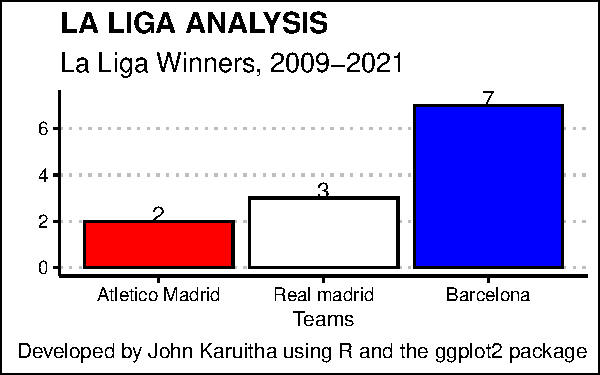
\includegraphics{web_scrapping_la_liga_files/figure-latex/graph_top_teams_2009_20-1}

\begin{Shaded}
\begin{Highlighting}[]
\DocumentationTok{\#\#\#\#\#\#\#\#\#\#\#\#\#\#\#\#\#\#\#\#\#\#\#\#\#\#\#\#\#\#\#\#\#\#\#\#\#\#\#\#\#\#\#\#}
\end{Highlighting}
\end{Shaded}

\hypertarget{conclusion}{%
\subsection{\texorpdfstring{\textbf{Conclusion}}{Conclusion}}\label{conclusion}}

Web scraping is a valuable skill in every researcher's toolkit, more so
with the rise of social media research. However, most scrapped data can
be messy and may require substantial effort cleaning. In this write-up,
I used \texttt{R} to demonstrate web scrapping. Other programming
languages like \texttt{Python} do offer the same capabilities.

\hypertarget{appendix}{%
\subsection{\texorpdfstring{\textbf{Appendix}}{Appendix}}\label{appendix}}

\hypertarget{appendix-1-la-liga-standings-2009-2021}{%
\subsubsection{Appendix 1: la Liga Standings
2009-2021}\label{appendix-1-la-liga-standings-2009-2021}}

\begin{Shaded}
\begin{Highlighting}[]
\DocumentationTok{\#\#\#\#\#\#\#\#\#\#\#\#\#\#\#\#\#\#\#\#\#\#\#\#\#\#\#\#\#\#\#\#\#\#\#\#\#\#\#\#\#\#\#\#}

\DocumentationTok{\#\# Appendix: The full list of data scrapped}

\NormalTok{la\_liga\_09\_2020}
\end{Highlighting}
\end{Shaded}

\begin{verbatim}
## $year2020
## # A tibble: 20 x 10
##      pos team               pl     w     d     l     f     a    gd   pts
##    <int> <chr>           <int> <int> <int> <int> <int> <int> <int> <int>
##  1     1 Atletico Madrid    38    26     8     4    67    25    42    86
##  2     2 Real Madrid        38    25     9     4    67    28    39    84
##  3     3 Barcelona          38    24     7     7    85    38    47    79
##  4     4 Sevilla            38    24     5     9    53    33    20    77
##  5     5 Real Sociedad      38    17    11    10    59    38    21    62
##  6     6 Real Betis         38    17    10    11    50    50     0    61
##  7     7 Villarreal         38    15    13    10    60    44    16    58
##  8     8 Celta Vigo         38    14    11    13    55    57    -2    53
##  9     9 Granada            38    13     7    18    47    65   -18    46
## 10    10 Athletic Bilbao    38    11    13    14    46    42     4    46
## 11    11 Osasuna            38    11    11    16    37    48   -11    44
## 12    12 Cadiz              38    11    11    16    36    58   -22    44
## 13    13 Valencia           38    10    13    15    50    53    -3    43
## 14    14 Levante            38     9    14    15    46    57   -11    41
## 15    15 Getafe             38     9    11    18    28    43   -15    38
## 16    16 Alaves             38     9    11    18    36    57   -21    38
## 17    17 Elche              38     8    12    18    34    55   -21    36
## 18    18 SD Huesca          38     7    13    18    34    53   -19    34
## 19    19 Real Valladolid    38     5    16    17    34    57   -23    31
## 20    20 Eibar              38     6    12    20    29    52   -23    30
## 
## $year2019
## # A tibble: 20 x 10
##      pos team               pl     w     d     l     f     a    gd   pts
##    <int> <chr>           <int> <int> <int> <int> <int> <int> <int> <int>
##  1     1 Real Madrid        38    26     9     3    70    25    45    87
##  2     2 Barcelona          38    25     7     6    86    38    48    82
##  3     3 Atletico Madrid    38    18    16     4    51    27    24    70
##  4     4 Sevilla            38    19    13     6    54    34    20    70
##  5     5 Villarreal         38    18     6    14    63    49    14    60
##  6     6 Real Sociedad      38    16     8    14    56    48     8    56
##  7     7 Granada            38    16     8    14    52    45     7    56
##  8     8 Getafe             38    14    12    12    43    37     6    54
##  9     9 Valencia           38    14    11    13    46    53    -7    53
## 10    10 Osasuna            38    13    13    12    46    54    -8    52
## 11    11 Athletic Bilbao    38    13    12    13    41    38     3    51
## 12    12 Levante            38    14     7    17    47    53    -6    49
## 13    13 Real Valladolid    38     9    15    14    32    43   -11    42
## 14    14 Eibar              38    11     9    18    39    56   -17    42
## 15    15 Real Betis         38    10    11    17    48    60   -12    41
## 16    16 Alaves             38    10     9    19    34    59   -25    39
## 17    17 Celta Vigo         38     7    16    15    37    49   -12    37
## 18    18 Leganes            38     8    12    18    30    51   -21    36
## 19    19 Real Mallorca      38     9     6    23    40    65   -25    33
## 20    20 Espanyol           38     5    10    23    27    58   -31    25
## 
## $year2018
## # A tibble: 20 x 10
##      pos team               pl     w     d     l     f     a    gd   pts
##    <int> <chr>           <int> <int> <int> <int> <int> <int> <int> <int>
##  1     1 Barcelona          38    26     9     3    90    36    54    87
##  2     2 Atletico Madrid    38    22    10     6    55    29    26    76
##  3     3 Real Madrid        38    21     5    12    63    46    17    68
##  4     4 Valencia           38    15    16     7    51    35    16    61
##  5     5 Getafe             38    15    14     9    48    35    13    59
##  6     6 Sevilla            38    17     8    13    62    47    15    59
##  7     7 Espanyol           38    14    11    13    48    50    -2    53
##  8     8 Athletic Bilbao    38    13    14    11    41    45    -4    53
##  9     9 Real Sociedad      38    13    11    14    45    46    -1    50
## 10    10 Real Betis         38    14     8    16    44    52    -8    50
## 11    11 Alaves             38    13    11    14    39    50   -11    50
## 12    12 Eibar              38    11    14    13    46    50    -4    47
## 13    13 Leganes            38    11    12    15    37    43    -6    45
## 14    14 Villarreal         38    10    14    14    49    52    -3    44
## 15    15 Levante            38    11    11    16    59    66    -7    44
## 16    16 Real Valladolid    38    10    11    17    32    51   -19    41
## 17    17 Celta Vigo         38    10    11    17    53    62    -9    41
## 18    18 Girona             38     9    10    19    37    53   -16    37
## 19    19 SD Huesca          38     7    12    19    43    65   -22    33
## 20    20 Rayo Vallecano     38     8     8    22    41    70   -29    32
## 
## $year2017
## # A tibble: 20 x 10
##      pos team                   pl     w     d     l     f     a    gd   pts
##    <int> <chr>               <int> <int> <int> <int> <int> <int> <int> <int>
##  1     1 Barcelona              38    28     9     1    99    29    70    93
##  2     2 Atletico Madrid        38    23    10     5    58    22    36    79
##  3     3 Real Madrid            38    22    10     6    94    44    50    76
##  4     4 Valencia               38    22     7     9    65    38    27    73
##  5     5 Villarreal             38    18     7    13    57    50     7    61
##  6     6 Real Betis             38    18     6    14    60    61    -1    60
##  7     7 Sevilla                38    17     7    14    49    58    -9    58
##  8     8 Getafe                 38    15    10    13    42    33     9    55
##  9     9 Eibar                  38    14     9    15    44    50    -6    51
## 10    10 Girona                 38    14     9    15    50    59    -9    51
## 11    11 Espanyol               38    12    13    13    36    42    -6    49
## 12    12 Real Sociedad          38    14     7    17    66    59     7    49
## 13    13 Celta Vigo             38    13    10    15    59    60    -1    49
## 14    14 Alaves                 38    15     2    21    40    50   -10    47
## 15    15 Levante                38    11    13    14    44    58   -14    46
## 16    16 Athletic Bilbao        38    10    13    15    41    49    -8    43
## 17    17 Leganes                38    12     7    19    34    51   -17    43
## 18    18 Deportivo La Coruna    38     6    11    21    38    76   -38    29
## 19    19 Las Palmas             38     5     7    26    24    74   -50    22
## 20    20 Malaga                 38     5     5    28    24    61   -37    20
## 
## $year2016
## # A tibble: 20 x 10
##      pos team                   pl     w     d     l     f     a    gd   pts
##    <int> <chr>               <int> <int> <int> <int> <int> <int> <int> <int>
##  1     1 Real Madrid            38    29     6     3   106    41    65    93
##  2     2 Barcelona              38    28     6     4   116    37    79    90
##  3     3 Atletico Madrid        38    23     9     6    70    27    43    78
##  4     4 Sevilla                38    21     9     8    69    49    20    72
##  5     5 Villarreal             38    19    10     9    56    33    23    67
##  6     6 Real Sociedad          38    19     7    12    59    53     6    64
##  7     7 Athletic Bilbao        38    19     6    13    53    43    10    63
##  8     8 Espanyol               38    15    11    12    49    50    -1    56
##  9     9 Alaves                 38    14    13    11    41    43    -2    55
## 10    10 Eibar                  38    15     9    14    56    51     5    54
## 11    11 Malaga                 38    12    10    16    49    55    -6    46
## 12    12 Valencia               38    13     7    18    56    65    -9    46
## 13    13 Celta Vigo             38    13     6    19    53    69   -16    45
## 14    14 Las Palmas             38    10     9    19    53    74   -21    39
## 15    15 Real Betis             38    10     9    19    41    64   -23    39
## 16    16 Deportivo La Coruna    38     8    12    18    43    61   -18    36
## 17    17 Leganes                38     8    11    19    36    55   -19    35
## 18    18 Sporting Gijon         38     7    10    21    42    72   -30    31
## 19    19 Osasuna                38     4    10    24    40    94   -54    22
## 20    20 Granada                38     4     8    26    30    82   -52    20
## 
## $year2015
## # A tibble: 20 x 10
##      pos team                   pl     w     d     l     f     a    gd   pts
##    <int> <chr>               <int> <int> <int> <int> <int> <int> <int> <int>
##  1     1 Barcelona              38    29     4     5   112    29    83    91
##  2     2 Real Madrid            38    28     6     4   110    34    76    90
##  3     3 Atletico Madrid        38    28     4     6    63    18    45    88
##  4     4 Villarreal             38    18    10    10    44    35     9    64
##  5     5 Athletic Bilbao        38    18     8    12    58    45    13    62
##  6     6 Celta Vigo             38    17     9    12    51    59    -8    60
##  7     7 Sevilla                38    14    10    14    51    50     1    52
##  8     8 Malaga                 38    12    12    14    38    35     3    48
##  9     9 Real Sociedad          38    13     9    16    45    48    -3    48
## 10    10 Real Betis             38    11    12    15    34    52   -18    45
## 11    11 Las Palmas             38    12     8    18    45    53    -8    44
## 12    12 Valencia               38    11    11    16    46    48    -2    44
## 13    13 Espanyol               38    12     7    19    40    74   -34    43
## 14    14 Eibar                  38    11    10    17    49    61   -12    43
## 15    15 Deportivo La Coruna    38     8    18    12    45    61   -16    42
## 16    16 Granada                38    10     9    19    46    69   -23    39
## 17    17 Sporting Gijon         38    10     9    19    40    62   -22    39
## 18    18 Rayo Vallecano         38     9    11    18    52    73   -21    38
## 19    19 Getafe                 38     9     9    20    37    67   -30    36
## 20    20 Levante                38     8     8    22    37    70   -33    32
## 
## $year2014
## # A tibble: 20 x 10
##      pos team                   pl     w     d     l     f     a    gd   pts
##    <int> <chr>               <int> <int> <int> <int> <int> <int> <int> <int>
##  1     1 Barcelona              38    30     4     4   110    21    89    94
##  2     2 Real Madrid            38    30     2     6   118    38    80    92
##  3     3 Atletico Madrid        38    23     9     6    67    29    38    78
##  4     4 Valencia               38    22    11     5    70    32    38    77
##  5     5 Sevilla                38    23     7     8    71    45    26    76
##  6     6 Villarreal             38    16    12    10    48    37    11    60
##  7     7 Athletic Bilbao        38    15    10    13    42    41     1    55
##  8     8 Celta Vigo             38    13    12    13    47    44     3    51
##  9     9 Malaga                 38    14     8    16    42    48    -6    50
## 10    10 Espanyol               38    13    10    15    47    51    -4    49
## 11    11 Rayo Vallecano         38    15     4    19    46    68   -22    49
## 12    12 Real Sociedad          38    11    13    14    44    51    -7    46
## 13    13 Elche                  38    11     8    19    35    62   -27    41
## 14    14 Levante                38     9    10    19    34    67   -33    37
## 15    15 Getafe                 38    10     7    21    33    64   -31    37
## 16    16 Deportivo La Coruna    38     7    14    17    35    60   -25    35
## 17    17 Granada                38     7    14    17    29    64   -35    35
## 18    18 Eibar                  38     9     8    21    34    55   -21    35
## 19    19 Almeria                38     8     8    22    35    64   -29    32
## 20    20 Cordoba                38     3    11    24    22    68   -46    20
## 
## $year2013
## # A tibble: 20 x 10
##      pos team               pl     w     d     l     f     a    gd   pts
##    <int> <chr>           <int> <int> <int> <int> <int> <int> <int> <int>
##  1     1 Atletico Madrid    38    28     6     4    77    26    51    90
##  2     2 Barcelona          38    27     6     5   100    33    67    87
##  3     3 Real Madrid        38    27     6     5   104    38    66    87
##  4     4 Athletic Bilbao    38    20    10     8    66    39    27    70
##  5     5 Sevilla            38    18     9    11    69    52    17    63
##  6     6 Villarreal         38    17     8    13    60    44    16    59
##  7     7 Real Sociedad      38    16    11    11    62    55     7    59
##  8     8 Valencia           38    13    10    15    51    53    -2    49
##  9     9 Celta Vigo         38    14     7    17    49    54    -5    49
## 10    10 Levante            38    12    12    14    35    43    -8    48
## 11    11 Malaga             38    12     9    17    39    46    -7    45
## 12    12 Rayo Vallecano     38    13     4    21    46    80   -34    43
## 13    13 Getafe             38    11     9    18    35    54   -19    42
## 14    14 Espanyol           38    11     9    18    41    51   -10    42
## 15    15 Granada            38    12     5    21    32    56   -24    41
## 16    16 Elche              38     9    13    16    30    50   -20    40
## 17    17 Almeria            38    11     7    20    43    71   -28    40
## 18    18 Osasuna            38    10     9    19    32    62   -30    39
## 19    19 Real Valladolid    38     7    15    16    38    60   -22    36
## 20    20 Real Betis         38     6     7    25    36    78   -42    25
## 
## $year2012
## # A tibble: 20 x 10
##      pos team                   pl     w     d     l     f     a    gd   pts
##    <int> <chr>               <int> <int> <int> <int> <int> <int> <int> <int>
##  1     1 Barcelona              38    32     4     2   115    40    75   100
##  2     2 Real Madrid            38    26     7     5   103    42    61    85
##  3     3 Atletico Madrid        38    23     7     8    65    31    34    76
##  4     4 Real Sociedad          38    18    12     8    70    49    21    66
##  5     5 Valencia               38    19     8    11    67    54    13    65
##  6     6 Malaga                 38    16     9    13    53    50     3    57
##  7     7 Real Betis             38    16     8    14    57    56     1    56
##  8     8 Rayo Vallecano         38    16     5    17    50    66   -16    53
##  9     9 Sevilla                38    14     8    16    58    54     4    50
## 10    10 Getafe                 38    13     8    17    43    57   -14    47
## 11    11 Levante                38    12    10    16    40    57   -17    46
## 12    12 Athletic Bilbao        38    12     9    17    44    65   -21    45
## 13    13 Espanyol               38    11    11    16    43    52    -9    44
## 14    14 Real Valladolid        38    11    10    17    49    58    -9    43
## 15    15 Granada                38    11     9    18    37    54   -17    42
## 16    16 Osasuna                38    10     9    19    33    50   -17    39
## 17    17 Celta Vigo             38    10     7    21    37    52   -15    37
## 18    18 Real Mallorca          38     9     9    20    43    72   -29    36
## 19    19 Deportivo La Coruna    38     8    11    19    47    70   -23    35
## 20    20 Real Zaragoza          38     9     7    22    37    62   -25    34
## 
## $year2011
## # A tibble: 20 x 10
##      pos team                pl     w     d     l     f     a    gd   pts
##    <int> <chr>            <int> <int> <int> <int> <int> <int> <int> <int>
##  1     1 Real Madrid         38    32     4     2   121    32    89   100
##  2     2 Barcelona           38    28     7     3   114    29    85    91
##  3     3 Valencia            38    17    10    11    59    44    15    61
##  4     4 Malaga              38    17     7    14    54    53     1    58
##  5     5 Atletico Madrid     38    15    11    12    53    46     7    56
##  6     6 Levante             38    16     7    15    54    50     4    55
##  7     7 Osasuna             38    13    15    10    44    61   -17    54
##  8     8 Real Mallorca       38    14    10    14    42    46    -4    52
##  9     9 Sevilla             38    13    11    14    48    47     1    50
## 10    10 Athletic Bilbao     38    12    13    13    49    52    -3    49
## 11    11 Getafe              38    12    11    15    40    51   -11    47
## 12    12 Real Sociedad       38    12    11    15    46    52    -6    47
## 13    13 Real Betis          38    13     8    17    47    56    -9    47
## 14    14 Espanyol            38    12    10    16    46    56   -10    46
## 15    15 Rayo Vallecano      38    13     4    21    53    73   -20    43
## 16    16 Real Zaragoza       38    12     7    19    36    61   -25    43
## 17    17 Granada             38    12     6    20    35    56   -21    42
## 18    18 Villarreal          38     9    14    15    39    53   -14    41
## 19    19 Sporting Gijon      38    10     7    21    42    69   -27    37
## 20    20 Racing Santander    38     4    15    19    28    63   -35    27
## 
## $year2010
## # A tibble: 20 x 10
##      pos team                   pl     w     d     l     f     a    gd   pts
##    <int> <chr>               <int> <int> <int> <int> <int> <int> <int> <int>
##  1     1 Barcelona              38    30     6     2    95    21    74    96
##  2     2 Real Madrid            38    29     5     4   102    33    69    92
##  3     3 Valencia               38    21     8     9    64    44    20    71
##  4     4 Villarreal             38    18     8    12    54    44    10    62
##  5     5 Sevilla                38    17     7    14    62    61     1    58
##  6     6 Athletic Bilbao        38    18     4    16    59    55     4    58
##  7     7 Atletico Madrid        38    17     7    14    62    53     9    58
##  8     8 Espanyol               38    15     4    19    46    55    -9    49
##  9     9 Osasuna                38    13     8    17    45    46    -1    47
## 10    10 Sporting Gijon         38    11    14    13    35    42    -7    47
## 11    11 Malaga                 38    13     7    18    54    68   -14    46
## 12    12 Racing Santander       38    12    10    16    41    56   -15    46
## 13    13 Real Zaragoza          38    12     9    17    40    53   -13    45
## 14    14 Levante                38    12     9    17    41    52   -11    45
## 15    15 Real Sociedad          38    14     3    21    49    66   -17    45
## 16    16 Getafe                 38    12     8    18    49    60   -11    44
## 17    17 Real Mallorca          38    12     8    18    41    56   -15    44
## 18    18 Deportivo La Coruna    38    10    13    15    31    47   -16    43
## 19    19 Hercules               38     9     8    21    36    60   -24    35
## 20    20 Almeria                38     6    12    20    36    70   -34    30
## 
## $year2009
## # A tibble: 20 x 10
##      pos team                   pl     w     d     l     f     a    gd   pts
##    <int> <chr>               <int> <int> <int> <int> <int> <int> <int> <int>
##  1     1 Barcelona              38    31     6     1    98    24    74    99
##  2     2 Real Madrid            38    31     3     4   102    35    67    96
##  3     3 Valencia               38    21     8     9    59    40    19    71
##  4     4 Sevilla                38    19     6    13    65    49    16    63
##  5     5 Real Mallorca          38    18     8    12    59    44    15    62
##  6     6 Getafe                 38    17     7    14    58    48    10    58
##  7     7 Villarreal             38    16     8    14    58    57     1    56
##  8     8 Athletic Bilbao        38    15     9    14    50    53    -3    54
##  9     9 Atletico Madrid        38    13     8    17    57    61    -4    47
## 10    10 Deportivo La Coruna    38    13     8    17    35    49   -14    47
## 11    11 Espanyol               38    11    11    16    29    46   -17    44
## 12    12 Osasuna                38    11    10    17    37    46    -9    43
## 13    13 Almeria                38    10    12    16    43    55   -12    42
## 14    14 Real Zaragoza          38    10    11    17    46    64   -18    41
## 15    15 Sporting Gijon         38     9    13    16    36    51   -15    40
## 16    16 Racing Santander       38     9    12    17    42    59   -17    39
## 17    17 Malaga                 38     7    16    15    42    48    -6    37
## 18    18 Tenerife               38     9     9    20    40    74   -34    36
## 19    19 Real Valladolid        38     7    15    16    37    62   -25    36
## 20    20 Xerez                  38     8    10    20    38    66   -28    34
\end{verbatim}

\begin{Shaded}
\begin{Highlighting}[]
\DocumentationTok{\#\#\#\#\#\#\#\#\#\#\#\#\#\#\#\#\#\#\#\#\#\#\#\#\#\#\#\#\#\#\#\#\#\#\#\#\#\#\#\#\#\#\#\#}
\end{Highlighting}
\end{Shaded}

\hypertarget{appendix-2-la-liga-top-3-teams-and-top-scorers-1929-2021}{%
\subsection{Appendix 2: La Liga Top 3 Teams and Top Scorers
1929-2021}\label{appendix-2-la-liga-top-3-teams-and-top-scorers-1929-2021}}

\begin{table}
\centering
\begin{tabular}{l|l|l|l|l|l|l}
\hline
season & winners & runners\_up & third\_place & top\_scorer\_s & top\_scorers\_club\_s & goals\\
\hline
1929 & Barcelona & Real Madrid (1) & Athletic Bilbao & Paco Bienzobas & Real Sociedad & 14\\
\hline
1929–30 & Athletic Bilbao & Barcelona (1) & Arenas & Guillermo Gorostiza & Athletic Bilbao & 19\\
\hline
1930–31 & Athletic Bilbao & Racing Santander (1) & Real Sociedad & Bata & Athletic Bilbao & 27\\
\hline
1931–32 & Real Madrid & Athletic Bilbao (1) & Barcelona & Guillermo Gorostiza & Athletic Bilbao & 12\\
\hline
1932–33 & Real Madrid & Athletic Bilbao (2) & Espanyol & Manuel Olivares & Real Madrid & 16\\
\hline
1933–34 & Athletic Bilbao & Real Madrid (2) & Racing Santander & Isidro Lángara & Oviedo & 27\\
\hline
1934–35 & Real Betis & Real Madrid (3) & Oviedo & Isidro Lángara & Oviedo & 26\\
\hline
1935–36 & Athletic Bilbao & Real Madrid (4) & Oviedo & Isidro Lángara & Oviedo & 27\\
\hline
1936–37 & Spanish Civil War (League Cancelled) & Spanish Civil War (League Cancelled) & Spanish Civil War (League Cancelled) & Spanish Civil War (League Cancelled) & Spanish Civil War (League Cancelled) & Spanish Civil War (League Cancelled)\\
\hline
1937–38 & Spanish Civil War (League Cancelled) & Spanish Civil War (League Cancelled) & Spanish Civil War (League Cancelled) & Spanish Civil War (League Cancelled) & Spanish Civil War (League Cancelled) & Spanish Civil War (League Cancelled)\\
\hline
1938–39 & Spanish Civil War (League Cancelled) & Spanish Civil War (League Cancelled) & Spanish Civil War (League Cancelled) & Spanish Civil War (League Cancelled) & Spanish Civil War (League Cancelled) & Spanish Civil War (League Cancelled)\\
\hline
1939–40 & Atlético Aviación[a] & Sevilla (1) & Athletic Bilbao & Víctor Unamuno & Athletic Bilbao & 22\\
\hline
1940–41 & Atlético Aviación[a] & Athletic Bilbao (3) & Valencia & Pruden & Atlético Aviación & 30\\
\hline
1941–42 & Valencia & Real Madrid (5) & Atlético Aviación & Edmundo Suárez & Valencia & 27\\
\hline
1942–43 & Athletic Bilbao & Sevilla (2) & Barcelona & Mariano Martín & Barcelona & 32\\
\hline
1943–44 & Valencia & Atlético Aviación (1) & Sevilla & Edmundo Suárez & Valencia & 27\\
\hline
1944–45 & Barcelona & Real Madrid (6) & Atlético Aviación & Telmo Zarra & Atlético Bilbao & 19\\
\hline
1945–46 & Sevilla & Barcelona (2) & Athletic Bilbao & Telmo Zarra & Atlético Bilbao & 24\\
\hline
1946–47 & Valencia & Athletic Bilbao (4) & Atlético Aviación & Telmo Zarra & Atlético Bilbao & 34\\
\hline
1947–48 & Barcelona & Valencia (1) & Atlético Madrid & Pahiño & Celta Vigo & 23\\
\hline
1948–49 & Barcelona & Valencia (2) & Real Madrid & César Rodríguez Álvarez & Barcelona & 28\\
\hline
1949–50 & Atlético Madrid & Deportivo La Coruña (1) & Valencia & Telmo Zarra & Athletic Bilbao & 25\\
\hline
1950–51 & Atlético Madrid & Sevilla (3) & Valencia & Telmo Zarra & Athletic Bilbao & 38\\
\hline
1951–52 & Barcelona & Athletic Bilbao (5) & Real Madrid & Pahiño & Real Madrid & 28\\
\hline
1952–53 & Barcelona & Valencia (3) & Real Madrid & Telmo Zarra & Athletic Bilbao & 24\\
\hline
1953–54 & Real Madrid & Barcelona (3) & Valencia & Alfredo Di Stéfano & Real Madrid & 27\\
\hline
1954–55 & Real Madrid & Barcelona (4) & Athletic Bilbao & Juan Arza & Sevilla & 28\\
\hline
1955–56 & Athletic Bilbao & Barcelona (5) & Real Madrid & Alfredo Di Stéfano & Real Madrid & 24\\
\hline
1956–57 & Real Madrid  † & Sevilla (4) & Barcelona & Alfredo Di Stéfano & Real Madrid & 31\\
\hline
1957–58 & Real Madrid  † & Atlético Madrid (2) & Barcelona & Manuel BadenesAlfredo Di StéfanoRicardo & ValladolidReal MadridValencia & 19\\
\hline
1958–59 & Barcelona & Real Madrid (7) & Athletic Bilbao & Alfredo Di Stéfano & Real Madrid & 23\\
\hline
1959–60 & Barcelona & Real Madrid (8) & Athletic Bilbao & Ferenc Puskás & Real Madrid & 26\\
\hline
1960–61 & Real Madrid & Atlético Madrid (3) & Zaragoza & Ferenc Puskás & Real Madrid & 27\\
\hline
1961–62 & Real Madrid & Barcelona (6) & Atlético Madrid & Juan Seminario & Zaragoza & 25\\
\hline
1962–63 & Real Madrid & Atlético Madrid (4) & Oviedo & Ferenc Puskás & Real Madrid & 26\\
\hline
1963–64 & Real Madrid & Barcelona (7) & Real Betis & Ferenc Puskás & Real Madrid & 20\\
\hline
1964–65 & Real Madrid & Atlético Madrid (5) & Zaragoza & Cayetano Ré & Barcelona & 25\\
\hline
1965–66 & Atlético Madrid & Real Madrid (9) & Barcelona & Vavá & Elche & 19\\
\hline
1966–67 & Real Madrid & Barcelona (8) & Espanyol & Waldo Machado & Valencia & 24\\
\hline
1967–68 & Real Madrid & Barcelona (9) & Las Palmas & Fidel Uriarte & Athletic Bilbao & 22\\
\hline
1968–69 & Real Madrid & Las Palmas (1) & Barcelona & Amancio AmaroJosé Eulogio Gárate & Real MadridAtlético Madrid & 14\\
\hline
1969–70 & Atlético Madrid & Athletic Bilbao (6) & Sevilla & Amancio AmaroLuis AragonésJosé Eulogio Gárate & Real MadridAtlético MadridAtlético Madrid & 16\\
\hline
1970–71 & Valencia & Barcelona (10) & Atlético Madrid & José Eulogio GárateCarles Rexach & Atlético MadridBarcelona & 17\\
\hline
1971–72 & Real Madrid & Valencia (4) & Barcelona & Enrique Porta & Granada & 20\\
\hline
1972–73 & Atlético Madrid & Barcelona (11) & Espanyol & Marianín & Oviedo & 19\\
\hline
1973–74 & Barcelona & Atlético Madrid (6) & Zaragoza & Quini & Sporting Gijón & 20\\
\hline
1974–75 & Real Madrid & Zaragoza (1) & Barcelona & Carlos & Athletic Bilbao & 19\\
\hline
1975–76 & Real Madrid & Barcelona (12) & Atlético Madrid & Quini & Sporting Gijón & 21\\
\hline
1976–77 & Atlético Madrid & Barcelona (13) & Athletic Bilbao & Mario Kempes & Valencia & 24\\
\hline
1977–78 & Real Madrid & Barcelona (14) & Athletic Bilbao & Mario Kempes & Valencia & 28\\
\hline
1978–79 & Real Madrid & Sporting Gijón (1) & Atlético Madrid & Hans Krankl & Barcelona & 29\\
\hline
1979–80 & Real Madrid & Real Sociedad (1) & Sporting Gijón & Quini & Sporting Gijón & 24\\
\hline
1980–81 & Real Sociedad & Real Madrid (10) & Atlético Madrid & Quini & Barcelona & 20\\
\hline
1981–82 & Real Sociedad & Barcelona (15) & Real Madrid & Quini & Barcelona & 26\\
\hline
1982–83 & Athletic Bilbao & Real Madrid (11) & Atlético Madrid & Hipólito Rincón & Real Betis & 20\\
\hline
1983–84 & Athletic Bilbao & Real Madrid (12) & Barcelona & Jorge da SilvaJuanito & ValladolidReal Madrid & 17\\
\hline
1984–85 & Barcelona & Atlético Madrid (7) & Athletic Bilbao & Hugo Sánchez & Atlético Madrid & 19\\
\hline
1985–86 & Real Madrid  ‡ & Barcelona (16) & Athletic Bilbao & Hugo Sánchez & Real Madrid & 22\\
\hline
1986–87 & Real Madrid & Barcelona (17) & Espanyol & Hugo Sánchez & Real Madrid & 34\\
\hline
1987–88 & Real Madrid & Real Sociedad (2) & Atlético Madrid & Hugo Sánchez & Real Madrid & 29\\
\hline
1988–89 & Real Madrid & Barcelona (18) & Valencia & Baltazar & Atlético Madrid & 35\\
\hline
1989–90 & Real Madrid & Valencia (5) & Barcelona & Hugo Sánchez & Real Madrid & 38\\
\hline
1990–91 & Barcelona & Atlético Madrid (8) & Real Madrid & Emilio Butragueño & Real Madrid & 19\\
\hline
1991–92 & Barcelona  † & Real Madrid (13) & Atlético Madrid & Manolo & Atlético Madrid & 27\\
\hline
1992–93 & Barcelona & Real Madrid (14) & Deportivo La Coruña & Bebeto & Deportivo La Coruña & 29\\
\hline
1993–94 & Barcelona & Deportivo La Coruña (2) & Zaragoza & Romário & Barcelona & 30\\
\hline
1994–95 & Real Madrid & Deportivo La Coruña (3) & Real Betis & Iván Zamorano & Real Madrid & 28\\
\hline
1995–96 & Atlético Madrid & Valencia (6) & Barcelona & Juan Antonio Pizzi & Tenerife & 31\\
\hline
1996–97 & Real Madrid & Barcelona (19) & Deportivo La Coruña & Ronaldo & Barcelona & 34\\
\hline
1997–98 & Barcelona & Athletic Bilbao (7) & Real Sociedad & Christian Vieri & Atlético Madrid & 24\\
\hline
1998–99 & Barcelona & Real Madrid (15) & Mallorca & Raúl & Real Madrid & 25\\
\hline
1999–2000 & Deportivo La Coruña & Barcelona (20) & Valencia & Salva Ballesta & Racing Santander & 27\\
\hline
2000–01 & Real Madrid & Deportivo La Coruña (4) & Mallorca & Raúl & Real Madrid & 24\\
\hline
2001–02 & Valencia & Deportivo La Coruña (5) & Real Madrid & Diego Tristán & Deportivo La Coruña & 21\\
\hline
2002–03 & Real Madrid & Real Sociedad (3) & Deportivo La Coruña & Roy Makaay & Deportivo La Coruña & 29\\
\hline
2003–04 & Valencia  ‡ & Barcelona (21) & Deportivo La Coruña & Ronaldo & Real Madrid & 25\\
\hline
2004–05 & Barcelona & Real Madrid (16) & Villarreal & Diego Forlán & Villarreal & 25\\
\hline
2005–06 & Barcelona  † & Real Madrid (17) & Valencia & Samuel Eto'o & Barcelona & 26\\
\hline
2006–07 & Real Madrid & Barcelona (22) & Sevilla & Ruud van Nistelrooy & Real Madrid & 25\\
\hline
2007–08 & Real Madrid & Villarreal (1) & Barcelona & Daniel Güiza & Mallorca & 27\\
\hline
2008–09 & Barcelona & Real Madrid (18) & Sevilla & Diego Forlán & Atlético Madrid & 32\\
\hline
2009–10 & Barcelona & Real Madrid (19) & Valencia & Lionel Messi & Barcelona & 34\\
\hline
2010–11 & Barcelona  † & Real Madrid (20) & Valencia & Cristiano Ronaldo & Real Madrid & 40\\
\hline
2011–12 & Real Madrid & Barcelona (23) & Valencia & Lionel Messi & Barcelona & 50\\
\hline
2012–13 & Barcelona & Real Madrid (21) & Atlético Madrid & Lionel Messi & Barcelona & 46\\
\hline
2013–14 & Atlético Madrid & Barcelona (24) & Real Madrid & Cristiano Ronaldo & Real Madrid & 31\\
\hline
2014–15 & Barcelona & Real Madrid (22) & Atlético Madrid & Cristiano Ronaldo & Real Madrid & 48\\
\hline
2015–16 & Barcelona & Real Madrid (23) & Atlético Madrid & Luis Suárez & Barcelona & 40\\
\hline
2016–17 & Real Madrid  † & Barcelona (25) & Atlético Madrid & Lionel Messi & Barcelona & 37\\
\hline
2017–18 & Barcelona & Atlético Madrid (9) & Real Madrid & Lionel Messi & Barcelona & 34\\
\hline
2018–19 & Barcelona & Atlético Madrid (10) & Real Madrid & Lionel Messi & Barcelona & 36\\
\hline
2019–20 & Real Madrid & Barcelona (26) & Atlético Madrid & Lionel Messi & Barcelona & 25\\
\hline
2020–21 & Atlético Madrid & Real Madrid (24) & Barcelona & Lionel Messi & Barcelona & 30\\
\hline
\end{tabular}
\end{table}

\bibliography{skeleton.bib}



\end{document}
